\documentclass{rapportECN}
\title{RAPPORT BAYES} %Titre du fichier


\usepackage{listings}
\usepackage{booktabs}
\usepackage{rotating}
\usepackage{graphicx} 
\usepackage{mwe} 
\usepackage{adjustbox}
\usepackage{minted}
\usepackage{tabularx}
\usepackage {tikz}
\usetikzlibrary {positioning}
\usetikzlibrary{calc}
\usepackage{bbm}

\begin{document}

%----------- Informations du rapport ---------

\titre{Rapport Bayes} %Titre du fichier .pdf
%\UE{PIIA} %Nom de l'UE
\sujet{BAYES} %Nom du sujet
\enseignant{Mathieu \textsc{RIBATET}} %Nom de l'enseignant
\eleves{Tom \textsc{MAYE-LASSERRE} \\
        Jérôme \textsc{FAUCHEUX}
		} %Nom des élèves

%----------- Initialisation -------------------
        
\fairemarges %Afficher les marges
\fairepagedegarde %Créer la page de garde
%\tabledematieres %Créer la table de matières

%------------ Corps du rapport ----------------

\section{Modèle Mathématiques}

Les données présentées sont celle d'une étude médicale sur la prise d'un traitement pour traiter les contractions ventilatoires prématurées (PVC).
On dispose de deux variables observées : 
\begin{itemize}
    \item $x_i$: PVC par minute avant la prise du traitement.
    \item $y_i$ PVC par minute après la prise du traitement.
\end{itemize}

Les hypothèse de modélisations conduisent au modèle suivant : 

\begin{equation} \label{eq1}
\begin{split}
    & x_i \sim \mathcal P (\lambda_i) \\
    & y_i \sim \mathcal P (\beta \lambda_i) \text{ pour les patients non gueris par le traitement}
\end{split}
\end{equation}

$\beta$ représente alors, pour les patients non guéris, la modification moyenne des PVC due à la prise du médicament (accélération si $\beta > 1$, diminution si $\beta < 1$).

On suppose toutes les variables aléatoires $(x_i)$ et $(y_i)$ indépendantes entre elles.

De plus, on modélise la probabilité d'être guéri par le traitement par une loi binomiale de paramètre $\theta$ : $\{\text{guerison du patient } i \} \sim \mathcal B(\theta)$.

La difficulté de cette modélisation vient des $\lambda_i$, différents pour chaque patients. Cependant, il est possible de montrer que :

\begin{equation}
    P(y_i \mid\{\text{non guerison du patient }i\} \cap x_i+y_i) \sim \mathcal{B}ern \left (\dfrac{\beta}{1 + \beta}, x_i+y_i \right) 
\end{equation}
Cette formule est beaucoup plus pratique, car elle ne fait intervenir que le paramètre $\beta$. À l'aide de ces formules, on propose alors les deux modèles suivants pour notre problème :

\begin{figure}[H]
\centering
\begin{minipage}[b]{0.4\textwidth}
\begin{center}
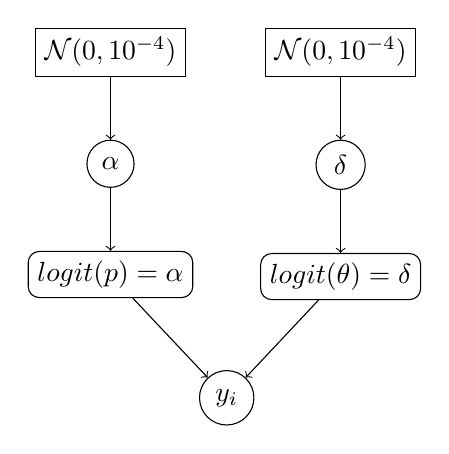
\begin{tikzpicture}

    \node[draw, rectangle] (N1) { $\mathcal{N}(0, 10^{-4})$ };
    \node[draw, rectangle, right=1cm of N1] (N2) { $\mathcal{N}(0, 10^{-4})$ };

    \node[draw, circle, below=0.8cm of N1] (alpha) { $\alpha$ };
    \node[draw, circle, below=0.8cm of N2] (delta) { $\delta$ };

    \node[draw, rounded corners, below=0.8cm of alpha] (logitp) { $logit( p) = \alpha$ };
    \node[draw, rounded corners, below=0.8cm of delta] (logittheta) { $logit( \theta) = \delta$ };

    \path (logitp) -- (logittheta) coordinate[midway] (midpoint);

    \node[draw, circle, below=1.2cm of midpoint] (yi) { $y_i$ };

    \draw[->] (N1) -- (alpha);
    \draw[->] (N2) -- (delta);
    \draw[->] (alpha) -- (logitp);
    \draw[->] (delta) -- (logittheta);
    \draw[->] (logitp) -- (yi);
    \draw[->] (logittheta) -- (yi);

\end{tikzpicture}
\end{center}
\end{minipage}
\hfill
\begin{minipage}[b]{0.4\textwidth}
\begin{center}
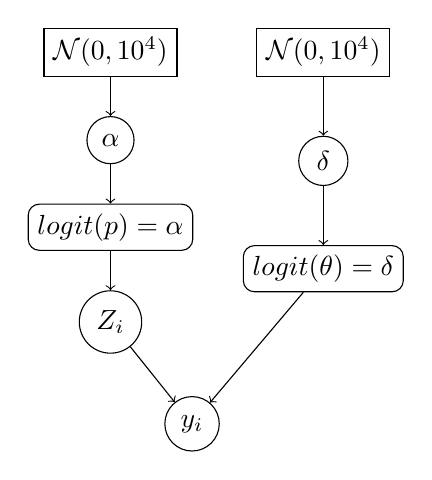
\begin{tikzpicture}

    \node[draw, rectangle] (N1) { $\mathcal{N}(0, 10^{4})$ };
    \node[draw, rectangle, right=1cm of N1] (N2) { $\mathcal{N}(0, 10^{4})$ };

    \node[draw, circle, below=0.5cm of N1] (alpha) { $\alpha$ };
    \node[draw, circle, below=0.75cm of N2] (delta) { $\delta$ };

    \node[draw, rounded corners, below=0.5cm of alpha] (logitp) { $logit( p) = \alpha$ };
    \node[draw, rounded corners, below=0.75cm of delta] (logittheta) { $logit( \theta) = \delta$ };
    \node[draw, circle, below=0.5cm of logitp](Zi) {$Z_i$};

    \path (Zi) -- (logittheta) coordinate[midway] (midpoint);

    \node[draw, circle, below=1.2cm of midpoint] (yi) { $y_i$ };

    \draw[->] (N1) -- (alpha);
    \draw[->] (N2) -- (delta);
    \draw[->] (alpha) -- (logitp);
    \draw[->] (delta) -- (logittheta);
    \draw[->] (logitp) -- (Zi);
    \draw[->] (Zi) -- (yi);
    \draw[->] (logittheta) -- (yi);

\end{tikzpicture}
\end{center}
\end{minipage}
\end{figure}

Le premier modèle est le plus simple d'un point, dans le sens où il est celui qui fait intervenir le moins de variables. On peut retrouver les équations de ce modèle dans la partie 1 du notebook associée. Le second modèle fait intervenir les variables latentes $Z_i$, qui représente l'état du patient $i$ (1 pour guéri, 0 pour non guéri). Là encore, les équations de ce modèle peuvent êtres trouvées dans le notebook associés. Ce modèle a été introduit dans l'espoir de simplifier les équations du premier modèle. En effet sachant $Z_i$, on a alors que $P(y_i \mid Z_i, \dots)$ est ou bien une variable aléatoire constante (0 si le patient est guéri, i.e. si $Z_i=1$), ou bien suit une loi de Bernoulli de paramètres $p$ et $t_i := x_i + y_i$.
Bien que cela simplifie la loi de $y_i \mid \dots$, cela nous ne permet pas de retomber pour les lois de $\alpha \mid \dots$ et $\delta \mid \dots$ sur des lois usuelles (notamment à cause du logit), et fournit donc au final un modèle très similaire, mais plus complexe que le premier modèle.

\section{Résultats}

On présente tout d'abord les résultats obtenus dans l'étude originale :

\begin{center}
\begin{tabular}{c | c  c  c}
& mean & sd & median \\
\hline
$\alpha$ & -0.4809 & 0.2795 & -0.4767 \\
$\beta$ & 0.6427 & 0.1812 & 0.6208 \\
$\delta$ & 0.3144 & 0.6177 & 0.3124 \\
$\theta$ & 0.5717 & 0.1391 & 0.5775 \\
\end{tabular}
\end{center}

Ceux ci correspondent à une chaîne de taille 10 000 avec une période de chauffe de 1000. Nous allons reproduire cette expérience pour nos deux modèles.

\subsection{Premier Modèle}

\begin{figure}[H]
\begin{minipage}{0.4\linewidth}
    \begin{center}
    \begin{tabular}{c | c  c  c}
    & mean & sd & median \\
    \hline
    $\alpha$ & -0.5075 & 0.2804 & -0.5067 \\
    $\beta$ & 0.6260  &  0.1778 & 0.6025 \\
    $\delta$ & 0.3690  &  0.7033  &  0.3467 \\
    $\theta$ & 0.5817  &  0.1535  &  0.5858 \\
    \end{tabular}
    \end{center}
\end{minipage}
\hfill
\begin{minipage}{0.5\linewidth}
    \includegraphics[width=1\linewidth]{figure/model1.png}
\end{minipage}
\end{figure}

Les chaînes ont un très bel aspect, et on obtient des taux de mélanges très raisonnables. (Le seul raffinement qu'il resterait à faire serait de proposer des déviations standards pour les noyaux différentes, on voit que celle de delta est un peu trop élevée, ainsi que le taux d'acceptation qui est de 0.6, contre 0.3 pour alpha, mais cela n'est pas dramatique). De plus on obtient des résultats très similaires à ceux de l'étude originale, ce qui nous conforte dans la bonne réalisation de nos algorithmes.

\subsection{Second Modèle}

\begin{figure}[H]
\begin{minipage}{0.4\linewidth}
    \begin{center}
    \begin{tabular}{c | c  c  c}
    & mean & sd & median \\
    \hline
    $\alpha$ & -0.5071  &  0.2824  & -0.4972 \\
    $\beta$ & 0.6266   & 0.1789  &  0.6082 \\
    $\delta$ & 0.3943  &  0.7280 &   0.3879 \\
    $\theta$ & 0.5866  &  0.1569  &  0.5958 \\
    \end{tabular}
    \end{center}
\end{minipage}
\hfill
\begin{minipage}{0.5\linewidth}
    \includegraphics[width=1\linewidth]{figure/model2.png}
\end{minipage}
\end{figure}

On observe que les deux modèles sont très similaires dans les résultats, et que les chaînes présentent elles aussi de bonnes caractéristiques (peut être la chaîne en $\delta$ oscille un peu trop). Cependant, on note numériquement quelques différences : 
\begin{itemize}
    \item Tout d'abord, pour obtenir des taux de mélanges raisonnables, il est nécessaire d’abaisser la déviation standard pour les noyaux par rapport au premier modèle (on pourrait même juger qu'ici elle n'a pas été assez abaissée, mais les résultats restent tout de même satisfaisant).
    \item Ensuite, en observant les valeurs moyennes des variables latentes, on se rends compte qu'elle ne change presque jamais d'états (ce qui est loin d'être étonnant pour certains patients du jeu de données, avec $y_i =0 $ et $x_i >> 1$).
\end{itemize}

Tous ces résultats nous montrent que bien que le second modèle reste corrects, la complexité qu'il rajoute n'est pas nécessaire pour modéliser le problème, et le premier modèle suffit largement.

Que ce soit pour le premier ou le second modèle, il n'est malheureusement pas possible de simuler des données à partir de nos paramètres, car cette étude n'a pas cherché à modéliser les $\lambda_i$, nécéssaire pour simuler les variables $x_i$ et $y_i$. Ainsi, nous ne pouvons pas pousser loin la vérification de nos modèles.

\subsection{Analyse des résultats}

Grâce à ces résultats numériques, on peut en déduire une action positive assez forte du médicament. Sous hypothèse de normalité asymptotique, on obtient que $\theta \in [0.58 \pm 0.003]$ avec probabilité d'au moins 95\%. Cela veut donc dire que le traitement soigne au moins la moitié des patients. De plus, pour les patients non guéris par le traitement, sous les mêmes hypothèses, on observe que $\beta \in [0.63 \pm 0.003]$. Là encore, cela sougigne un impact positif du traitement, puisque cela signifie une diminution moyenne de la fréquence des PVC de 40\%. 

Cependant, le jeu de données étant d'une taille vraiment faible (12 échantillons), cela ne permet pas de donner de forte garanties statistiques.
\include{annexe}

\end{document}
